\documentclass[12pt]{article}
\usepackage[english]{babel}

% \usepackage{amsmath, amssymb}
\usepackage{graphicx}
\usepackage{fancyhdr}
\usepackage{url}

\usepackage{tikz}
\usepackage{amsmath}
\usetikzlibrary{arrows}
\usepackage{verbatim}

\pagestyle{fancy}

\makeatletter

\begin{document}

\begin{titlepage}
\thispagestyle{plain}

\begin{center}
	
\includegraphics[scale=0.12]{unitnlogo}	\\
	University of Trento	\\
	\small {Department of Computer Science}	\\[1cm]
\end{center}

{\centering
\textbf{\Huge An algorithm implementation for Global Predicate Evaluation}\\[1cm]
% \small{Project for the “Distributed Algorithms” course}\\
\small{Trento, 29/08/2016}	\\[1cm]
\textbf{Zen Roberto \& Bof Michele}

}
\vfill

\section*{Abstract}

One core problem in distributed computing is to detect wheter a particular state in a computation can be reached and need to be detected. Problems such as deadlocks detection, monitoring or debugging can be all seen as an instance of the so called Global Predicate Evaluation (GPE) problem. This problem consists in evaluate wheter a given condition called predicate is satisfied among the consistent global states of the system. In order to solve it, one has to face all the practical issues that may arise in a distributed computation: asynchrony and failures of the underlying distributed system, message ordering and inconsistent observations. In this work, we present an implementation that solves GPE based on a simulation of a distributed system. The model built is based on message passing between peers and a monitor which passively observe the system in order to build its global states.


\end{titlepage}


\vspace{3cm}

\section{Introduction}

Aliqua eu exercitation mollit incididunt sunt labore in. Ut et Lorem non irure excepteur ad do laboris magna nostrud nostrud id minim eiusmod officia dolor. Pariatur sunt culpa ex do incididunt ad consequat officia cillum ex laboris. Occaecat occaecat labore sint reprehenderit aute pariatur sunt deserunt commodo pariatur in esse. Labore veniam nulla nisi esse sint aute pariatur ut commodo ipsum proident. Dolore quis quis quis commodo ad cupidatat elit in reprehenderit anim reprehenderit magna deserunt qui dolor officia. Eiusmod quis ad commodo laborum proident enim proident duis ad qui officia.

\subsection*{Motivation}

The reasons which have motivated our group to conduct a study on this topic are the following:

\begin{enumerate}
\item \textbf{Reason 1}. Enim aute ex ullamco eiusmod eu sit ullamco reprehenderit esse anim sint amet esse..
\item \textbf{Id cillum exercitation adipisicing incididunt commodo quis tempor labore.}. Id cillum exercitation adipisicing incididunt commodo quis tempor labore..
\item \textbf{Id cillum exercitation adipisicing incididunt commodo quis tempor labore.}. Id cillum exercitation adipisicing incididunt commodo quis tempor labore.
\end{enumerate}

\subsection*{Goals}

The objectives which we have set ourselves are the following:
\begin{enumerate}
\item \textbf{Simulate a distributed computation}. Structure the project in such a way that an user can define how the simulation has to be executed and and how long it has to last. Moreover how many peers run over it and configura the probability of executing and internal event rather than a message exchange.

\item \textbf{Id cillum exercitation adipisicing incididunt commodo quis tempor labore.}. Id cillum exercitation adipisicing incididunt commodo quis tempor labore..
\item \textbf{Id cillum exercitation adipisicing incididunt commodo quis tempor labore.}. Id cillum exercitation adipisicing incididunt commodo quis tempor labore.
\end{enumerate}


\subsection*{Results}

We developed a practical solution to the GPE problem based on a random simulation of distrubuted computations. The project has been develop in Java using JDK version's $1.7$ in combination with the Akka framework which allowed us to build an highly concurrent, distributed, and resilient message-driven application\footnote{\url{http://akka.io}}. We started implementing the behaviour of the peers and then we defined the message exchange between them. In particolar, we adopted a simple strategy for structure messages in a way that they were able to transport all the information needed at the very end of the simulation. To conclude, we defined the behaviour of the monitor such that it was able to collect all the messages exchanged between the peers and evaluate a given predicate over them building consistend global states stored in a lattice of events.

\subsection*{Outline}

The outline of this report is structured as follows. Section 2 describes the problem of GPE while Section 3 explains details about the solution we propose, the problems we faced and the strategies we adopted to overcome them. In Section 4 we will show some experimental evaluations of our implementation. The last section states the conclusion of our work and ideas on how we could improve our solution with techniques based on high-level operators that run in parallel.

\section{The Problem}

\section{The Solution}


At the end we decided to allow users to run a simulation of a distributed computation. Indeed, each execution of our implementation runs a simulation.

This section  gives readers all the competences to understand our proposed solution.

In this section we do not go deep into the implementation details, instead we will focus on the logics behind our strategies.

\subsection{Initialization}

Each simulation starts with a

\subsection{The simulation}

\tikzstyle{every picture}+=[remember picture]
\everymath{\displaystyle}
\begin{figure}[!ht]

\hspace{0.5cm} Events:
\([ \thinspace
\tikz\node [fill=red!20,draw,circle] (n1) {}; \thinspace
\tikz\node [fill=green!20,draw,circle] (n2){}; \thinspace
\tikz\node [fill=blue!20,draw,circle] (n3) {}; \thinspace
\tikz\node [fill=black!20,draw,circle] (n4){}; \thinspace
]
\vspace{1cm}
\)

\centering
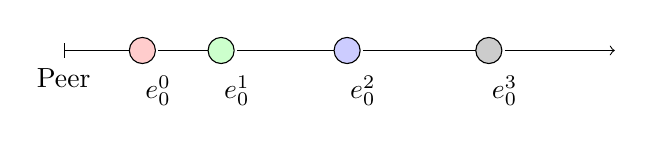
\begin{tikzpicture}
\draw[|-] (1,0) node[below=1mm]{Peer} -- (2,0) node{\tikz[baseline]{
	\node[fill=red!20,draw,circle] (e0){};
}};
\draw[-] (2.2,0) node[below=2mm]{$e^0_0$} -- (3,0) node{\tikz[baseline]{
	\node[fill=green!20,draw,circle] (e1){};
}};
\draw[-] (3.2,0) node[below=2mm]{$e^1_0$} -- (4.6,0) node{\tikz[baseline]{
	\node[fill=blue!20,draw,circle] (e2){};
}};
\draw[-] (4.8,0) node[below=2mm]{$e^2_0$} -- (6.4,0) node{\tikz[baseline]{
	\node[fill=black!20,draw,circle] (e3){};
}};
\draw[->] (6.6,0) node[below=2mm]{$e^3_0$} -- (8,0) node[below=1mm]{};
\end{tikzpicture}

\begin{tikzpicture}[overlay]
        \path[->] (n1) edge [out=-90, in=120] (e0);
        \path[->] (n2) edge [out=-90, in=120] (e1);
        \path[->] (n3) edge [out=-70, in=135] (e2);
        \path[->] (n4) edge [out=-60, in=135] (e3);
\end{tikzpicture}

  \caption{The sequence of events stored in the peer list's and scheduled in the time space diagram.}
	\label{fig:events}
\end{figure}


Non laborum excepteur sint sunt aute esse aliquip. Velit irure ea culpa nulla id mollit laboris laboris adipisicing ipsum non do in id aute anim cupidatat. Veniam deserunt excepteur commodo eu duis nulla adipisicing anim amet adipisicing ex. Laborum Lorem do nulla sint qui voluptate sint esse in incididunt Lorem cillum voluptate tempor nisi. Mollit voluptate mollit eiusmod anim elit nostrud voluptate veniam commodo id do officia cillum voluptate fugiat cillum. In incididunt proident qui id velit eiusmod aliquip aliqua nulla officia ut. Dolore aute est aliqua qui do eu sunt in est ad aliquip nulla anim deserunt. Ut sunt voluptate consectetur magna ex minim ut magna cillum aliquip elit voluptate ex excepteur eiusmod occaecat.

\pagestyle{empty}
\tikzstyle{every picture}+=[remember picture]
\everymath{\displaystyle}

\begin{figure}[!ht]

\centering
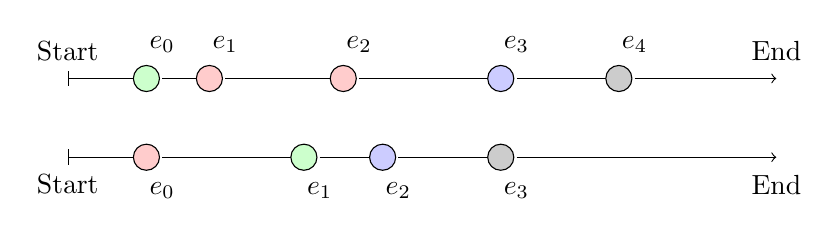
\begin{tikzpicture}

% FIRST TIMELINE

\draw[|-] (1,0) node[below=1mm]{Start} -- (2,0) node{\tikz[baseline]{
	\node[fill=red!20,draw,circle] (e0){};
}
};
\draw[-] (2.2,0) node[below=2mm]{$e_0$} -- (4,0) node{\tikz[baseline]{
	\node[fill=green!20,draw,circle] (e1){};
}
};
\draw[-] (4.2,0) node[below=2mm]{$e_1$} -- (5,0) node{\tikz[baseline]{
	\node[fill=blue!20,draw,circle] (e2){};
}
};
\draw[-] (5.2,0) node[below=2mm]{$e_2$} -- (6.5,0) node{\tikz[baseline]{
	\node[fill=black!20,draw,circle] (e3){};
}
};
\draw[->] (6.7,0) node[below=2mm]{$e_3$} -- (10,0) node[below=1mm]{End};

% SECOND TIMELINE

\draw[|-] (1,1) node[above=1mm]{Start} -- (2,1) node{\tikz[baseline]{
	\node[fill=green!20,draw,circle] (f0){};
}
};
\draw[-] (2.2,1) node[above=2mm]{$e_0$} -- (2.8,1) node{\tikz[baseline]{
	\node[fill=red!20,draw,circle] (f1){};
}
};
\draw[-] (3,1) node[above=2mm]{$e_1$} -- (4.5,1) node{\tikz[baseline]{
	\node[fill=red!20,draw,circle] (f2){};
}
};
\draw[-] (4.7,1) node[above=2mm]{$e_2$} -- (6.5,1) node{\tikz[baseline]{
	\node[fill=blue!20,draw,circle] (f3){};
}
};
\draw[-] (6.7,1) node[above=2mm]{$e_3$} -- (8,1) node{\tikz[baseline]{
	\node[fill=black!20,draw,circle] (f4){};
}
};
\draw[->] (8.2,1) node[above=2mm]{$e_4$} -- (10,1) node[above=1mm]{End};

\end{tikzpicture}

% Now it's time to draw some edges between the global nodes. Note that we
% have to apply the 'overlay' style.
\begin{tikzpicture}[overlay]
        \path[->] (f0) edge [out=-90, in=135] (e1);
        \path[->] (e2) edge [out=45, in=-135] (f3);
        \path[->] (e3) edge [out=45, in=-135] (f4);
\end{tikzpicture}

  \caption{An example of a simulation. Red circles are peers' internal events.}
\end{figure}


Non laborum excepteur sint sunt aute esse aliquip. Velit irure ea culpa nulla id mollit laboris laboris adipisicing ipsum non do in id aute anim cupidatat. Veniam deserunt excepteur commodo eu duis nulla adipisicing anim amet adipisicing ex. Laborum Lorem do nulla sint qui voluptate sint esse in incididunt Lorem cillum voluptate tempor nisi. Mollit voluptate mollit eiusmod anim elit nostrud volup.

\tikzstyle{every picture}+=[remember picture]
\everymath{\displaystyle}
\begin{figure}[ht!]
\centering
\scalebox{.8}{
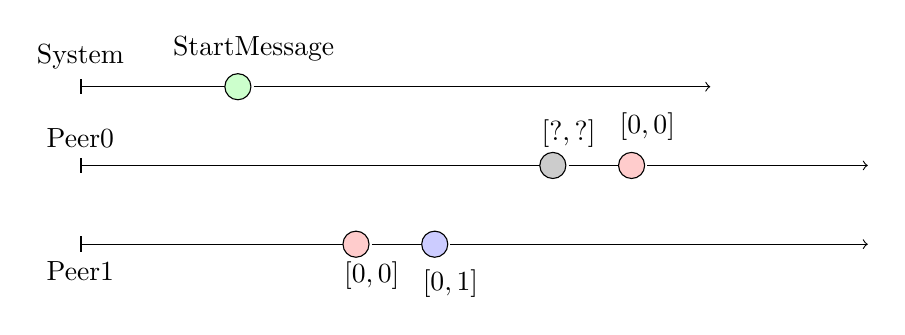
\begin{tikzpicture}

% SYSTEM
\draw[|-] (0,2) node[above=1mm]{System} -- (2,2) node{\tikz[baseline]{
	\node[fill=green!20,draw,circle] (sm){};
}};
\draw[->] (2.2,2) node[above=2mm]{StartMessage} -- (8,2) {};

% PEER 0
\draw[|-] (0,1) node[above=1mm]{Peer0} -- (6,1) node{\tikz[baseline]{
	\node[fill=black!20,draw,circle] (f0){};
}};
\draw[-] (6.2,1) node[above=1mm]{$[?,?]$} -- (7,1) node{\tikz[baseline]{
	\node[fill=red!20,draw,circle] (f1){};
}};
\draw[->] (7.2,1) node[above=2mm]{$[0,0]$} -- (10,1) node[below=1mm]{};

% PEER 1
\draw[|-] (0,0) node[below=1mm]{Peer1} -- (3.5,0) node{\tikz[baseline]{
	\node[fill=red!20,draw,circle] (e0){};
}};
\draw[-] (3.7,0) node[below=1mm]{$[0,0]$} -- (4.5,0) node{\tikz[baseline]{
	\node[fill=blue!20,draw,circle] (e1){};
}};
\draw[->] (4.7,0) node[below=2mm]{$[0,1]$} -- (10,0) node[below=1mm]{};

\end{tikzpicture}

\begin{tikzpicture}[overlay]
  \path[->] (sm) edge [out=-90, in=135] (e0);
  \path[->] (sm) edge [out=-45, in=135] (f1);
  \path[->] (e1) edge [out=45, in=-135] (f0);
\end{tikzpicture}
}

\caption{An overcomed issue in our asyncronous simulation.}
\label{fig:worst_case}
\end{figure}


Non laborum excepteur sint sunt aute esse aliquip. Velit irure ea culpa nulla id mollit laboris laboris adipisicing ipsum non do in id aute anim cupidatat. Veniam deserunt excepteur commodo eu duis nulla adipisicing anim amet adipisicing ex. Laborum Lorem do nulla sint qui voluptate sint esse in incididunt Lorem cillum voluptate tempor nisi. Mollit voluptate mollit eiusmod anim elit nostrud volup

\section{Evaluation}

\section{Conclusion}

\section{References}

\end{document}
